\documentclass[]{ximera}
%handout:  for handout version with no solutions or instructor notes
%handout,instructornotes:  for instructor version with just problems and notes, no solutions
%noinstructornotes:  shows only problem and solutions

%% handout
%% space
%% newpage
%% numbers
%% nooutcomes

%I added the commands here so that I would't have to keep looking them up
%\newcommand{\RR}{\mathbb R}
%\renewcommand{\d}{\,d}
%\newcommand{\dd}[2][]{\frac{d #1}{d #2}}
%\renewcommand{\l}{\ell}
%\newcommand{\ddx}{\frac{d}{dx}}
%\everymath{\displaystyle}
%\newcommand{\dfn}{\textbf}
%\newcommand{\eval}[1]{\bigg[ #1 \bigg]}

%\begin{image}
%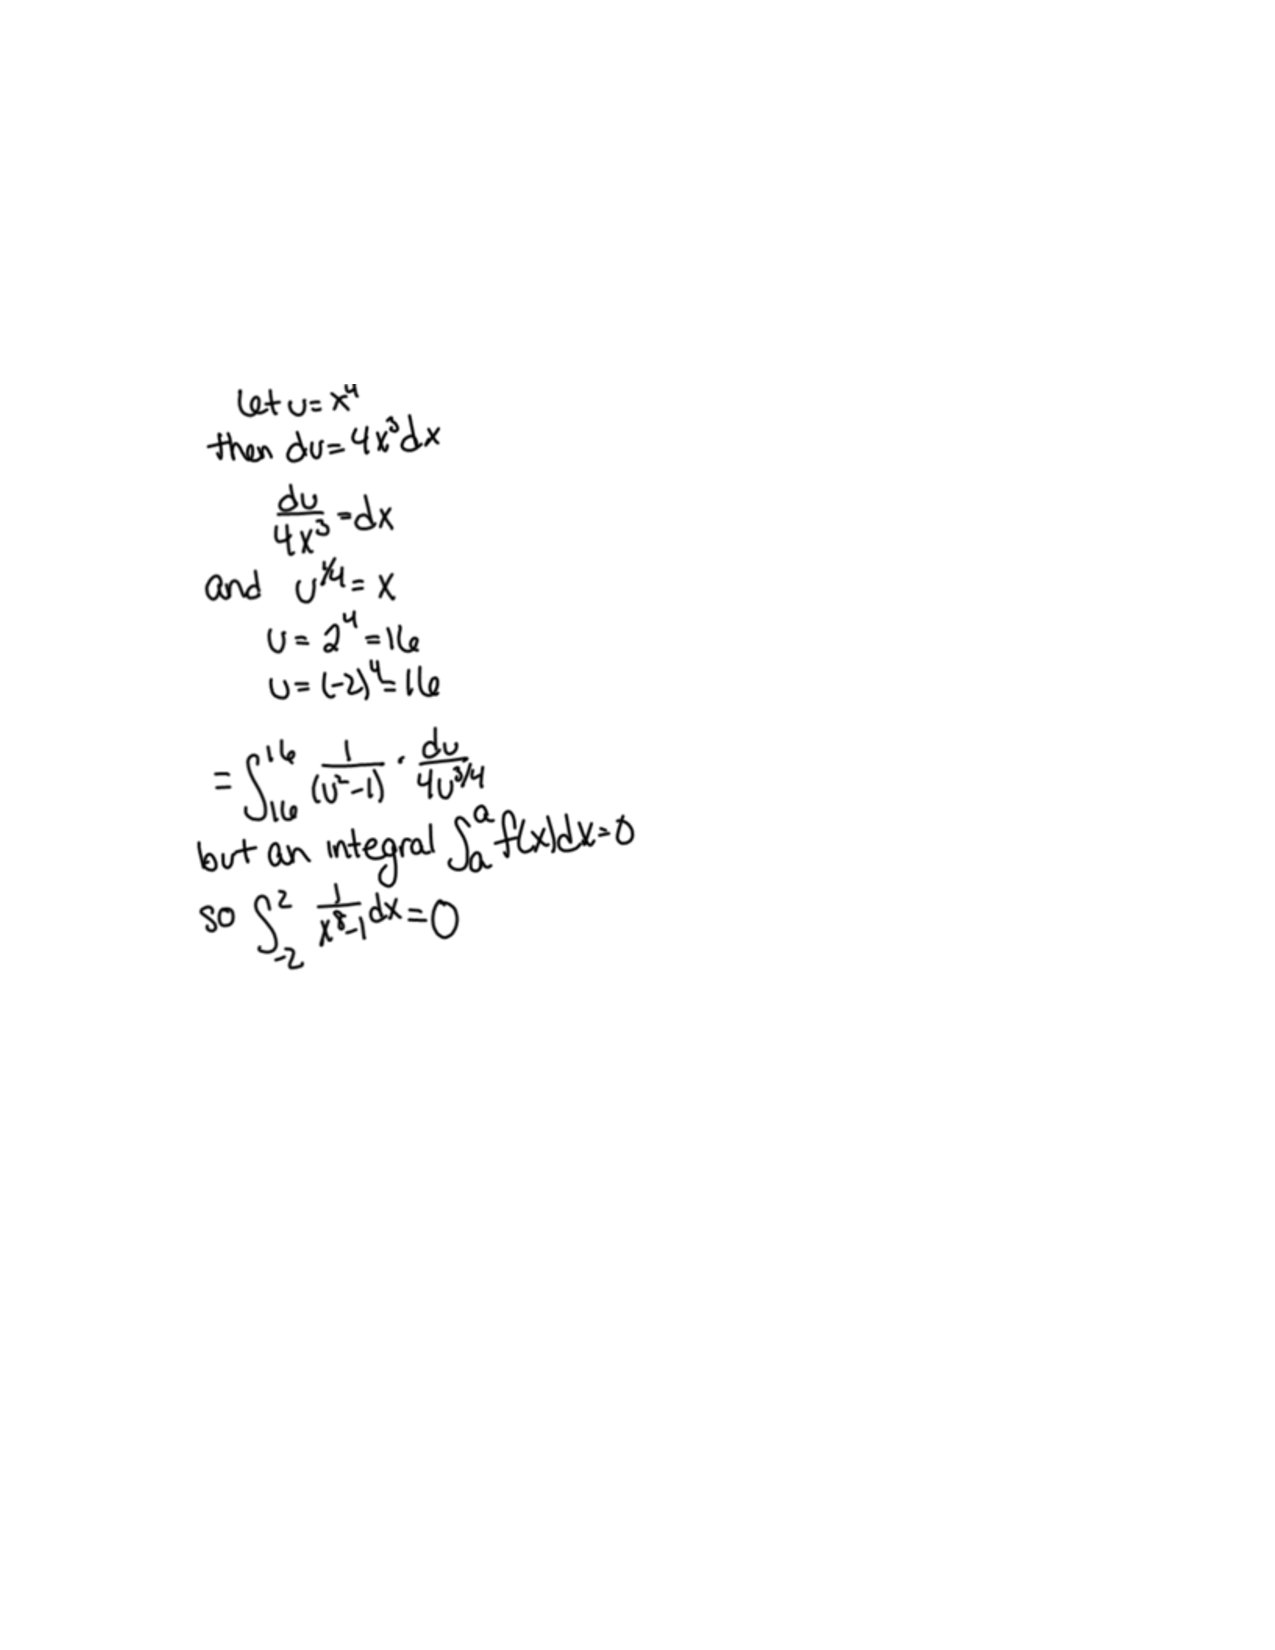
\includegraphics[trim= 170 420 250 180]{Figure1.pdf}
%\end{image}

%add a ``.'' below when used in a specific directory.
\newcommand{\RR}{\mathbb R}
\renewcommand{\d}{\,d}
\newcommand{\dd}[2][]{\frac{d #1}{d #2}}
\renewcommand{\l}{\ell}
\newcommand{\ddx}{\frac{d}{dx}}
\newcommand{\dfn}{\textbf}
\newcommand{\eval}[1]{\bigg[ #1 \bigg]}

\usepackage{multicol}

\renewenvironment{freeResponse}{
\ifhandout\setbox0\vbox\bgroup\else
\begin{trivlist}\item[\hskip \labelsep\bfseries Solution:\hspace{2ex}]
\fi}
{\ifhandout\egroup\else
\end{trivlist}
\fi} %% we can turn off input when making a master document

\title{The divergence and integral tests}  

\begin{document}
\begin{abstract}		\end{abstract}
\maketitle



\begin{comment}
\section{Warm up:}

	\begin{freeResponse}
	
	\end{freeResponse}
	
\begin{instructorNotes}

\end{instructorNotes}
\end{comment}







\section{Group work:}



%problem 1
\begin{problem}
For each of the following, answer {\bf True} or {\bf False}, and explain why.
	\begin{enumerate}
	
	\item  If $\sum_{n=0}^\infty a_n$ converges, then $\sum_{n=0}^\infty (a_n + 0.001)$ converges.
	
	\item  Since $\int_1^\infty x \sin(\pi x) \d x$ diverges then, by the Integral Test, $\sum_{n=0}^\infty n \sin(\pi n)$ diverges.
	
	\item  Since $\int_1^\infty \frac{1}{x^2} \d x = 1$ then, by the Integral Test, $\sum_{k=1}^\infty \frac{1}{k^2} = 1$.  
	
	\end{enumerate}
	
	\begin{freeResponse}
		\begin{enumerate}
		
		\item  {\bf False}
		
		Since $\sum_{n=0}^\infty a_n$ converges, we know that $\lim_{n \to \infty} a_n = 0$.  
		But then 
			\[
			\lim_{n \to \infty} (a_n + 0.0001) = 0.0001 \neq 0
			\]
		and so $\sum_{n=0}^\infty (a_n + 0.001)$ diverges by the Divergence Test.
		
		
		
		\item  {\bf False}
		
		The Integral Test only holds for positive, decreasing functions.  
		The function $f(x)= x \sin(\pi x)$ is not always positive, nor is it always decreasing.  
		So the Integral Test does not apply here.
		
		This problem is simpler than that though.  
		Since $\sin(\pi n) = 0$ for all integers $n$, we have that $\sum_{n=0}^\infty n \sin(\pi n) = 0$.
		
		
		
		\item  {\bf False}
		
		The Integral Test tells us that $\sum_{k=1}^\infty \frac{1}{k^2}$ converges, but it does {\bf not} give us the sum (this sum is actually $\frac{\pi^2}{6}$).  
		
		\end{enumerate}
	\end{freeResponse}
	
\end{problem}

\begin{instructorNotes}
For part (b) we need $f(x)$ to be a decreasing function for the Integral Test to (necessarily) hold.
All groups should do all of the parts.
\end{instructorNotes}







%problem 2
\begin{problem}
Assume $\sum_{k=0}^\infty a_k =L$ and $b_k = 8$ for all $k$. 
	\begin{enumerate}
	
	\item  What is $\lim_{k \to \infty} (a_k + b_k)$?
	
	\item  What is $\lim_{k \to \infty} \sum_{n=0}^k (a_n + b_n)$?
	
	\item  What is $\lim_{k \to \infty} \sum_{n=0}^k (a_{n+1} - a_n)$?
	
	\end{enumerate}
	
	\begin{freeResponse}
		\begin{enumerate}
	
		\item  Since $\sum_{k=0}^\infty a_k$ converges, we know that $\lim_{k \to \infty} a_k = 0$.  
		Therefore,
			\[
			\lim_{k \to \infty} (a_k + b_k) = 0 + 8 = \boxed{8}.
			\]
	
		\item  Since $\lim_{n \to \infty} (a_n + b_n) = 8$, the series $\sum_{n=0}^\infty (a_n + b_n)$ diverges by the Divergence Test.  
		But $\lim_{k \to \infty}  \sum_{n=0}^k (a_n + b_n) = \sum_{n=0}^\infty (a_n + b_n)$.  
		Thus
			\[
			\lim_{k \to \infty}  \sum_{n=0}^k (a_n + b_n) = \sum_{n=0}^\infty (a_n + b_n) = \boxed{\infty}.
			\]
	
		\item  Let $S_k = \sum_{n=0}^k (a_{n+1} - a_n)$ (and recall that $\{ S_k \}$ is the {\it sequence of partial sums}).
		Then
			\begin{align*}
			S_k &= \sum_{n=0}^k (a_{n+1} - a_n)  \\
			&= (a_1 - a_0) + (a_2 - a_1) + (a_3 - a_2) + \hdots + (a_k - a_{k-1}) + (a_{k+1} - a_k)  \\
			&= a_{k+1} - a_0.
			\end{align*}
		Thus,
			\[
			\lim_{k \to \infty} \sum_{n=0}^k (a_{n+1} - a_n) = \lim_{k \to \infty} S_k = \lim_{k \to \infty} a_{k+1} - a_0 = \boxed{-a_0}.
			\]
	
		\end{enumerate}
	\end{freeResponse}
		
\end{problem}

\begin{instructorNotes}
This question was adapted from midterm \#2 in Spring 2013.  
Students had difficulty distinguishing between a question dealing with sequences vs. a question dealing with series.
\end{instructorNotes}







\begin{comment}
%problem 3
\begin{problem}

	\begin{freeResponse}
	
	\end{freeResponse}

\end{problem}

\begin{instructorNotes}

\end{instructorNotes}
\end{comment}
















	
	
	
	
	
	
	
	
	

	










								
				
				
	














\end{document} 


















